\chapter{Kiến thức cơ sở xác suất và thống kê}\label{ch:1}
\section{Biến ngẫu nhiên và xác suất}\label{sec:1.1}
Biến ngẫu nhiên là một hàm ánh xạ với đặc điểm nó gán một giá trị bằng số cho kết quả đầu ra của một phép thử ngẫu nhiên.
\begin{align}
    \textbf{x}(\omega)=\textit{x}
\end{align}
với $\omega$ là đại diện cho đầu ra của một thực nghiệm, \textit{x} là một số thực (hay sự kiện), \textbf{x} là hàm ánh xạ (hay biến ngẫu nhiên).  
Tính ngẫu nhiên được thể hiện ở tham số đầu vào $\omega$. Điều này dẫn đến đầu ra của hàm là ngẫu nhiên.\\
Đây chưa phải là định nghĩa đầy đủ của một biến ngẫu nhiên. Khái niệm khác liên quan đến định nghĩa của một biến ngẫu nhiên là khái niệm xác suất. \\
Xét một số thí dụ sau:
\begin{itemize}
    \item Gieo một đồng xu trên mặt phẳng, đây là một phép thử. Kết quả có thể xảy ra là \textit{Xuất hiện mặt sấp} hoặc \textit{Xuất hiện mặt ngửa}. Như vậy xác suất cho các khả năng \textit{Xuất hiện mặt sấp} và \textit{Xuất hiện mặt ngửa} lần lượt là 
	$ \frac{1}{2} $ và $ \frac{1}{2} $
	\begin{figure}[H]
		\centering
		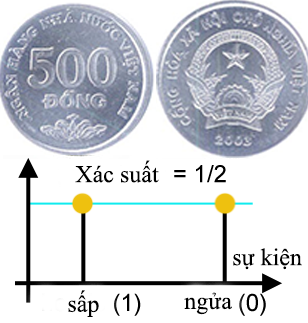
\includegraphics[width=0.4\textwidth]{coin.png}
		\caption{Các sự kiện có thể xuất hiện khi gieo đồng xu}
	   \end{figure}
    \item Gieo một con súc sắc, đây là một phép thử. Kết quả có thể xảy ra là "Xuất hiện mặt k chấm" tương ứng với k = 1,2,3,..,6. Xác suất cho mỗi sự kiện "Xuất hiện k chấm" đều là $ \frac{1}{6} $.
    \begin{figure}[H]
		\centering
		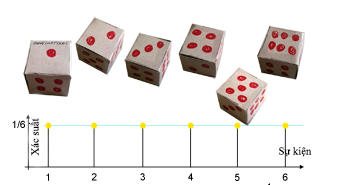
\includegraphics[width=0.6\textwidth]{xucxac.png}
		\caption{Các sự kiện có thể xuất hiện khi gieo súc sắc}
	   \end{figure}
\end{itemize}
Tổng quát, nếu một phép thử tạo ra n sự kiện khác nhau và khả năng xảy ra như nhau thì xác suất của mỗi sự kiện là $ \frac{1}{n} $
chúng ta có thể nói rằng nếu kết quả của một quá trình nào đó phải là một trong n kết quả khác nhau. 
\par
\section{Phân phối xác suất}\label{sec:1.2}
Phân phối xác suất xác định xác suất cho từng sự kiện có thể xảy ra của một phép thử ngẫu nhiên. Hàm phân phối xác suất của biến ngẫu nhiên \textbf{x} được xác định như sau:
\begin{align}
	\textbf{F}(x)=\textbf{P}(\textbf{x}\leq\textit{x})=\textbf{P}\left\{{\omega\in\Omega:\textbf{x}(\Omega)\leq\textit{x}} \right\}
\end{align}
với mọi $\textit{x}\in\textbf{R}$ được gọi là hàm phân phối xác suất của biến ngẫu nhiên $\textbf{x}$.

Đặc trưng của hàm phân phối xác suất hay gọi là hàm phân phối tích luỹ (CDF)
là lấy xác suất các biến ngẫu nhiên bên trái của một giá trị \textbf{x} bất kì nào đó.
Hàm này có đặc điểm là một hàm không giảm, tức là nếu $\textit{a}<\textit{b}$
thì $\textbf{F}(a)\leq\textbf{F}(b)$ vì sự kiện $\textit{b}$ đã bao gồm cả sự kiện $\textit{a}$ rồi.
\par
\subsection{Hàm khối xác suất của biến rời rạc}\label{subsec:1.2.1}
Hàm xác xuất để xác định xác suất tại mỗi giá trị \textbf{x} nào đó trong miền giá trị là bao nhiêu.
Hàm xác xuất như vậy được gọi là hàm khối xác suất (PMF) Đối với các biến ngẫu nhiên rời rạc. 
Giả sử miền giá trị của $\textbf{x}$ là $\textbf{D}$, tức $\textbf{x}$:$\bf\Omega\mapsto$$\textbf{D}$ thì hàm khối xác suất được xác định như sau: 
\begin{equation}
	\textit{p}(x)=\textit{p}\textit{X}(\textit{x})=
	\begin{cases}
	\textbf{P}(\textbf{x}=\textit{x}) &if \textit{x}\in\textbf{D}\\
	0 &if \textit{x}\notin\textbf{D}
	\end{cases}
\end{equation}
Như vậy ta có thể thấy rằng hàm khối xác suất thực chất cũng là một xác suất nên nó mang đầy đủ tất cả các tính chất của xác suất như:
\begin{itemize}
	\item 0$\leq\textit{p}(x)\leq$1
	\item $\sum_{x_i\in\textbf{D}}\textit{p}(x_{i})=$1
\end{itemize}
\par
\subsection{Hàm mật độ xác suất của biến liên tục}\label{subsec:1.2.2}
Hàm mật độ xác suất (PDF - Probability Density Function) đối với các biến ngẫu nhiên liên tục, dùng để ước lượng độ tập trung xác suất tại lân cận điểm nào đó.
Hàm mật độ xác suất \textit{f}(\textit{x}) tại điểm \textit{x} được xác định bằng cách lấy đạo hàm của hàm phân phối tích lũy \textbf{F}(\textit{x}) tại điểm đó:
\begin{align}
	\textit{f}(x)=\textbf{F}'(x)
\end{align}
Như vậy thì nơi nào \textit{f}(\textit{x}) càng lớn thì ở đó mức độ tập xác suất càng cao. 
Từ đây ta cũng có thể biểu diễn hàm phân phối tích luỹ như sau: 
\begin{align}
	\textbf{F}(x)=\int_{-\infty}^{x}\textit{f}(t)dt
\end{align}
Xác suất trong 1 khoảng ($\alpha$,$\beta$) cũng có thể được tính bằng hàm mật độ xác suất: 
\begin{align}
	\textbf{F}(x)=\int_{\alpha}^{\beta}\textit{f}(x)dx
\end{align}
Hàm mật độ xác suất cũng có 2 tính chất như xác suất như sau:
\begin{itemize}
	\item Không âm: $\textit{f}(x)\geq$0, $\forall(x)\in\textbf{R}$
	\item Tổng toàn miền bằng 1: $\int_{-\infty}^{\infty}\textit{f}(x)\textit{dx}$=1
\end{itemize}
\par
\section{Kỳ vọng và phương sai}\label{sec:1.3}
Giá trị kỳ vọng của X là tổng “sự kiện” nhân với xác suất của sự kiện đó. Như đã nhắc đến phần $ \ref{sec:1.2} $, 
xác suất được tính theo hàm PMF cho biến ngẫu nhiên rời rạc và hàm PDF cho biến ngẫu nhiên liên tục. 
Hay nói cách khác giá trị kỳ vọng là giá trị trung bình có trọng số.
\begin{align}
	\textbf{E}[\textbf{x}]=\sum_{i=0}^{N-1}{X_ipmf(X_i)}
\end{align}
Trong đó N là số “\textit{sự kiện}” có thể xảy ra của một biến ngẫu nhiên rời rạc $\textbf{x}$. 
Để mở rộng cho biến ngẫu nhiên liên tục $\textbf{x}$: 
\begin{align}
	\textbf{E}[\textbf{x}]=\int_{-\infty}^{\infty}{\textbf{x}pdf(\textbf{x})}
\end{align}
Giả sử $\textbf{x}$ là một biến ngẫu nhiên có tập giá trị sau {1, 2, 3, 4, 5, 6} và $\textbf{F}[\textbf{x}]=(\textbf{x}-3)^2$. Chú ý rằng  $\textbf{x}$ là biến ngẫu nhiên thì $\textbf{E}[\textbf{x}]$ cũng là một biến ngẫu nhiên.
Như vậy
\begin{itemize}
	\centering
	\item $\textbf{x}=1,\textbf{F}(1)=(1-3)^2=4$
	\item $\textbf{x}=2,\textbf{F}(2)=(2-3)^2=1$
	\item $\textbf{x}=3,\textbf{F}(3)=(3-3)^2=0$
	\item $\textbf{x}=4,\textbf{F}(4)=(4-3)^2=1$
	\item $\textbf{x}=5,\textbf{F}(5)=(5-3)^2=4$
	\item $\textbf{x}=6,\textbf{F}(6)=(6-3)^2=9$
\end{itemize}
Nhận thấy, xác suất của một kết quả $\textbf{Y}$ từ $\textbf{F}[\textbf{x}]$ bằng tổng xác suất của bất kỳ X nào thỏa $\textbf{F}[\textbf{x}]=\textbf{Y}$.

\begin{itemize}
	\centering
	\item $\textbf{P}(\textbf{F}(0))=\frac{1}{6}$
	\item $\textbf{P}(\textbf{F}(1))=\frac{1}{6}+\frac{1}{6}=\frac{2}{6}$
	\item $\textbf{P}(\textbf{F}(4))=\frac{1}{6}+\frac{1}{6}=\frac{2}{6}$
	\item $\textbf{P}(\textbf{F}(9))=\frac{1}{6}$
\end{itemize}

Trong toán học có hai phương pháp để tính giá trị kỳ vọng của $\textbf{F}[\textbf{x}]$ 
\begin{itemize}
	\item Phương pháp 1: Nếu phân phối xác suất của $\textbf{F}[\textbf{x}]$ đã biết trước, thì giá trị kỳ vọng được tính như sau:
	\begin{align}
		\textbf{E}[\textbf{F}[\textbf{x}]]=\textbf{E}[\textbf{Y}]=\sum{Y_i\textbf{P}(Y_i)}
	\end{align}
	\item Phương pháp 2: Nếu phân phối xác suất của $\textbf{F}[\textbf{x}]$ chưa biết trước, thì giá trị kỳ vọng được tính như sau: 
	Đối với biến ngẫu nhiên rời rạc
	\begin{align}
		\textbf{E}[\textbf{F}(\textbf{x})]=\sum{\textbf{F}(\textbf{x})\textbf{P}(\textbf{x})}
	\end{align}
	Đối với biến ngẫu nhiên liên tục
	\begin{align}
		\textbf{E}[\textbf{F}(\textbf{x})]=\int{\textbf{F}(\textbf{x})\textbf{P}(\textbf{x})d\textbf{x}}
	\end{align}
\end{itemize}
Phương pháp 2 đóng vai trò quan trọng trong phương pháp Monte Carlo. 
Bởi vì hàm phân phối xác xuất $\textbf{F}(\textbf{x})$ có thể không được biết trước.
Phương sai được xác định như sau
\begin{align}
	\sigma^2[\textbf{Y}]=E[(\textbf{Y}-\textbf{E}[\textbf{Y}])^2]
\end{align}
trong đó $\sigma$, độ lệch chuẩn, là căn bậc hai của phương sai. 
Từ những định nghĩa này, nó là dễ dàng cho thấy rằng với bất kỳ hằng số a
\begin{align}
	\textbf{E}[a\textbf{Y}]=a\textbf{E}[\textbf{Y}]
\end{align}
\begin{align}
	\sigma^2[a\textbf{Y}]=a^2\sigma^2[\textbf{Y}]
\end{align}
Hơn nữa, giá trị kỳ vọng của một tổng các biến ngẫu nhiên Yi là tổng giá trị kỳ vọng của Yi:
\begin{align}
	E\left[\sum_i{Y_i}\right]=\sum_i{E[Y_i]}
\end{align}
Từ các tính chất này, có thể rút ra biểu thức đơn giản hơn cho phương sai:
\begin{align}
	\sigma^2[\textbf{Y}]=\textbf{E}[\textbf{Y}^2]-\textbf{E}[\textbf{Y}]^2
\end{align}
Ngoài ra, nếu các biến ngẫu nhiên độc lập thì:
\begin{align}
	\sigma^2\left[\sum_i{Y_i}\right]=\sum_i{\sigma^2[Y_i]}\label{ct1.17}
\end{align}
